
\documentclass[letterpaper,twocolumn,10pt]{usetex-v1}

\usepackage{times}
\usepackage{subfigure}
\usepackage{graphicx}
\usepackage{color}
\usepackage{endnotes}
\usepackage{listings}
%\usepackage{ulem}
\usepackage{wrapfig}
\usepackage{amsmath,amssymb}
\usepackage{makecell}
\usepackage{booktabs}
\usepackage{multirow}
\usepackage[hyphens]{url}
\usepackage{cite}
\usepackage{xfp}
\usepackage[colorlinks=true,linkcolor=black,citecolor=black,pdfborder={0 0 0}]{hyperref}
\usepackage{breakurl}
\usepackage{enumitem}
\usepackage[table]{xcolor}
\usepackage{xspace}
\usepackage{microtype}
\usepackage[font=small,labelfont=bf]{caption}
\usepackage{comment}
\usepackage{textcomp}
\usepackage{algorithm}
\usepackage[noend]{algpseudocode}
%\usepackage[linesnumbered,ruled,vlined]{algorithm2e}

\usepackage{tikz}
\usepackage{amsmath}
\usepackage{multicol}
\usepackage{graphicx}
\usepackage{caption}
\usepackage{graphicx}
\usepackage{pifont}
%\usepackage{subfig}
\usepackage{algorithm}
\usepackage{subfigure}
\usepackage{enumitem}
\usepackage{multirow}
\usepackage{pifont}
\usepackage{booktabs}
\usepackage{xspace}
\usepackage{cleveref}
\usepackage{xcolor}
\usepackage{fancyhdr} 
\crefname{section}{§}{§§}
\Crefname{section}{§}{§§}
%follows are new added

\usepackage[english]{babel}
\usepackage{blindtext}

\usepackage{pifont}

% hopefully embeds all fonts in pdf
\usepackage[T1]{fontenc}
\usepackage[utf8]{inputenc}
\usepackage{pslatex}

% use times math
\usepackage{mathptmx}
\DeclareMathAlphabet{\mathcal}{OMS}{cmsy}{m}{n}
\DeclareMathAlphabet{\mathrm}{OT1}{bch}{m}{n}
\DeclareMathAlphabet{\mathit}{OT1}{bch}{m}{it}

\setlength{\hoffset}{0in}
\setlength{\voffset}{0in}
\setlength{\oddsidemargin}{-0.25in}
\setlength{\evensidemargin}{-0.25in}
\setlength{\topmargin}{0in}
\setlength{\headheight}{0in}
\setlength{\headsep}{0in}
\setlength{\textwidth}{7in}
\setlength{\textheight}{9in}
\setlength{\marginparsep}{0pt}
\setlength{\marginparwidth}{0pt}
\setlength{\columnsep}{0.33in}

\setitemize{noitemsep,topsep=0em,parsep=0em,partopsep=3pt}

\newcommand{\cmark}{\ding{51}}
\pagestyle{plain}

%%%%%%%%%%%%%%%%%%%%%%%%%%%%%%%%%

\renewcommand{\paragraph}[1]{\smallskip\noindent {\bf #1}}
\renewcommand{\ttdefault}{cmtt}
\newcommand\sysname{\textsf{Hercules}\xspace}
\newcommand\incname{Pantheon\xspace}


% my package
\usepackage{colortbl}
\usepackage{enumitem}
\usepackage{multirow}
\usepackage{float}

% to be able to draw some self-contained figs
\usepackage{tikz}
\usepackage{amsmath}

% inlined bib file
\usepackage{filecontents}

%-------------------------------------------------------------------------------
\begin{document}
%-------------------------------------------------------------------------------

%don't want date printed
\date{}

% make title bold and 14 pt font (Latex default is non-bold, 16 pt)
\title{2023 Fall CSE 221 Operating Systems Group Project}

\author{{Yanbo Zhou, Xiaochuan Yu} \\ Group 6}

\maketitle
\section{Introduction}
\label{sec:intro}
In this project, our goal is to help other students to deeply understand computer systems including concepts and its associated behaviors. To achieve this goal, our group members, Yanbo Zhou and Xiaochuan Yu, will build specific measurement tools and conduct experiments on system-level. Furthermore, we will analyze our experimental results based on the computer system concepts.

Our measurement and experiments are conducted on AWS EC2 Instance. Note that since we use EC2 Instance that is a virtualized environment, the virtualization layer will introduce part of overhead for our experiments. Therefore, the results may include the Guest Operating System (OS) operations and underlying virtualization overhead. In this report, we focus on methodology on measuring computer system. You can also use the methodology and our provided tools on physical machines, in order to avoid the virtualization overhead on EC2 Instance.

In the rest of this report, we will first introduce our hardware description in Section~{\S\ref{sec:hardware}}. Then we talk about CPU, Scheduling, and OS Services in Section xx; Memory in Section xx; Network in Section xx; and File System in Section xx. Finally, we summarize our experiments and report in Section xx. Xiaochuan Yu is responsible for CPU, Scheduling, and OS Service, and Yanbo Zhou will be responsible for Memory and File System experiments.

\section{Hardware Description}
\label{sec:hardware}
We use AWS Cloud Instance~\cite{awsi4} for our project and experiments. The basic hardware configuration for our instance is as follows.

\paragraph{Processor.} The table below shows the processor description.
\begin{table}[h]
	\centering
	\begin{tabular}{c|c}
		\hline
		CPU Model & Intel Xeon Platinum 8259CL  \\ \hline
		
		CPU(s) & 2 vCPUs \\ \hline

		CPU MHz & 2.50GHz \\ \hline
		
		L1 data cache & 32 KiB \\ \hline
		L1 instruction cache & 32 KiB \\ \hline
		L2 cache & 1 MiB \\ \hline
		L3 cache & 35.8 MiB \\ \hline
		Architecture & x86\_64 \\ \hline
	\end{tabular}
	\caption{\textbf{Processor Description}}
	\label{table:sys-conf}
	%\vspace{-7mm}
\end{table}

\paragraph{Memory bus.} In our AWS Instance, we have a Physical Memory Array (PMA) in memory bus. The detailed configuration of the PMA is as follows:
\begin{itemize}[leftmargin=*]
	\item Location: System Board Or Motherboard
	\item Use: System Memory
	\item Error Correction Type: Unknown
	\item Maximum Capacity: 904 MiB
	\item Error Information Handle: Not Provided
	\item Number Of Devices: 1
\end{itemize}

\paragraph{I/O bus.} The following shows the detailed I/O bus configuration about our AWS Instance.
\begin{itemize}[leftmargin=*]
	\item Host bridge: Intel Corporation 440FX - 82441FX PMC
	\item ISA bridge: Intel Corporation 82371SB PIIX3 ISA 
	\item Non-VGA unclassified device: Intel Corporation
	\item VGA compatible controller: Amazon.com, Inc.
	\item Non-Volatile memory controller: Amazon.com, Inc. NVMe EBS Controller
	\item Ethernet controller: Amazon.com, Inc. Elastic Network Adapter (ENA)
\end{itemize}

\paragraph{Others.} The other hardware description is shown as follows:
\begin{table}[h]
	\centering
	\begin{tabular}{c|c}
		\hline
		Memory & 904MiB DDR4 DRAM \\ \hline
		
		Storage & NVMe SSD 8GB without cache \\ \hline

		Network & 28Gbps \\ \hline
		
		OS & Amazon Linux version 2022, release 2022 \\ \hline
	\end{tabular}
	\caption{\textbf{Experimental System Configuration.}}
	\label{table:sys-conf}
	%\vspace{-7mm}
\end{table}



\subsection{CPU, Scheduling, and OS Services}
In this section, we will measure the overhead of procedure call, system call, and the time of task creation and context switching.

\subsubsection{Procedure Call}
First we need to define the overhead of procedure call. We assert that the overhead of function calls stems from three key factors: 1. Preparation of function parameters; 2. The setup of the function's stack frame during the function call; 3. Function return. Considering the code in \ref{lst1}. 
\lstinputlisting[language=C++,label=lst1,caption={Non inline procedure call}]{assets/code/lst1.c}
In System V AMD64 ABI (todo: cite), when calling function, the caller needs to setup the arguments for the callee, then pushes the return address and stack base pointer to the stack and jumps to the callee. When callee returns to the caller it will recover the previous stack frame and pop the return address to the program counter register to back to the caller's code. Thus, we can define the overhead of a procudure call as the additional cost incurred by three components: parameter preparation, stack frame adjustment before the jump, and stack frame adjustment upon return. To measure this overhead, we can calculate the time it takes from invoking a simplest function to its return.
\lstinputlisting[label=lst2,caption={Simplest function takes only one argument}]{assets/code/simplest_func.asm}
By using the simplest function in \ref{lst2}, we can eliminate the performance impact brought about by compiler optimizations (e.g. inlining) and security features (e.g. stack canaries).

Before measuring procedure calls, we also need to figure out the calling conventions. In System V AMD64 ABI, Programs typically pass parameters as table \ref{table:calling-convention-reg}\footnote{We are using cdecl calling convention.}.
\begin{table}[h]
	\centering
	\begin{tabular}{c|c}
		\hline
		\bf{Arguments} & \bf{How they are passed} \\ \hline
		
		First 6 Integers & RDI, RSI, RDX, RCX, R8, R9 \\ \hline

		First 8 Floating Points & XMM0-XMM7 \\ \hline
		
		Others & Stack \\ \hline
	\end{tabular}
	\caption{\textbf{Arguments Passing in System V AMD64 Calling Convention.}}
	\label{table:calling-convention-reg}
\end{table}
From this, we can make an early prediction that, for procedure calls with integer parameters, there won't be a significant difference in calling overhead when the number of parameters is less than or equal 6. It's only when there are more than 6 parameters that significant differences may arise due to memory writes.

\paragraph{Measure the overhead.} To measure the overhead more precisely, we use rdtscp\footnote{In order to preserve the execution order, we use rdtscp instead of rdtsc} instruction (todo: cite) to read from the processor’s time-stamp counter in order to get the number of CPU cycles. In order to mitigate the impact of process scheduling, we call the same function consecutively multiple times. Also, we use setpriority() to raise the scheduling priority of our testing program. Before conducting the tests, we ensure that the size of the test program is smaller than a page and disable swap. This is done to maximize the likelihood of the program being fully loaded into memory during the testing process. Every testing procedure call will be executed 0x1000000 times. The result is listed in table \ref{table:procedure-test}
\begin{table}[h]
	\centering
	\begin{tabular}{c|c}
		\hline
		\bf{Arguments} & \bf{Average Cycles} \\ \hline
		0 & 50.617 \\ \hline
		1 & 50.971 \\ \hline
		2 & 47.398 \\ \hline
        3 & 50.075 \\ \hline
        4 & 52.003 \\ \hline
        5 & 51.180 \\ \hline
        6 & 49.692 \\ \hline
        7 & 57.141 \\ \hline
	\end{tabular}
	\caption{\textbf{Result of Overhead of Procedure Call.}}
	\label{table:procedure-test}
\end{table}
Also we remove the function calling to measure the overhead of rdtscp.
The average cycles is 45.260. This aligns closely with our previous predictions: when the number of parameters is between 0 and 6, there is no significant difference in overhead. It is only when memory access is required that a noticeable increase in overhead becomes apparent.

todo: more precisely measure this by sub the time spent in kernel mode.

\subsubsection{System Call}
The overhead of a syscall, as compared to a regular procedure call, primarily arises from the context switching. Therefore, our primary task is to ascertain when will syscalls, or more frequently encountered libc syscall wrappers for usermode programmers, genuinely trap into kernel mode.

\paragraph{Virtual Syscall.} Virtual Dynamic Shared Object, vDSO is a kernel mechanism for exporting a selected part of kernel space routines to user space. VDSO provides user mode programs with vsyscalls. These virtual syscalls eliminate the need for user mode programs to spend time on context switching for certain simple syscalls. They are the syscalls without really trapping into kernel.

\begin{lstlisting}[caption=vDSO mapping]
gef> vmmap
...
0xffffffffff600000 
0xffffffffff601000 
0x0000000000000000 --x [vsyscall]
\end{lstlisting}

\paragraph{Measure the overhead.} We choose a simple system, clock\_gettime() to measure the overhead. Since we have the vDSO mapping, subtracting the number of cycles required for a syscall from those needed for VDSO can provide an estimate of the overhead associated with context switching. The result is in table
\begin{table}[h]
	\centering
	\begin{tabular}{c|c}
		\hline
		\bf{syscall} & \bf{vDSO call} \\ \hline
        1517.221 & 63.588 \\ \hline
	\end{tabular}
	\caption{\textbf{Result of Overhead of Procedure Call.}}
	\label{table:procedure-test}
\end{table}
Thus the overhead of context switching can be calculated as follows:
\begin{equation}
t_{\textbf{syscall}}-t_{\textbf{vDSO}}=1453.633
\end{equation}

\section{Memory}
\label{sec:memory}
In this section, we will measure RAM access time, bandwidth, and page fault service time, respectively.

\subsection{RAM  Access Time}
\paragraph{Methodology.}
In this case, we first fill the memory array to 
warm up cache in different levels. Then, we measure latency by increasing 
access regions from 1KiB to 128MiB. Since L1/L2/L3 caches have limited capacity, only part
of data can be cached in different levels of cache so that we can measure the access time when
we increase access regions. However, the compiler optimization and cache prefetch may have influence
on final results. Therefore, we introduce two approaches to avoid the influence caused by the
compiler optimization and cache prefetch. On the one hand, we separate memory region into multiple
256KiB strips and randomly chain them into a link list to avoid cache line (64KiB) prefetch influence.
On the other hand, we touch the pointer when we measure latency and use GCC with "O0" parameter to avoid
compiler optimization.

\paragraph{Experimental results.}
\begin{figure}[t]
	\centering
	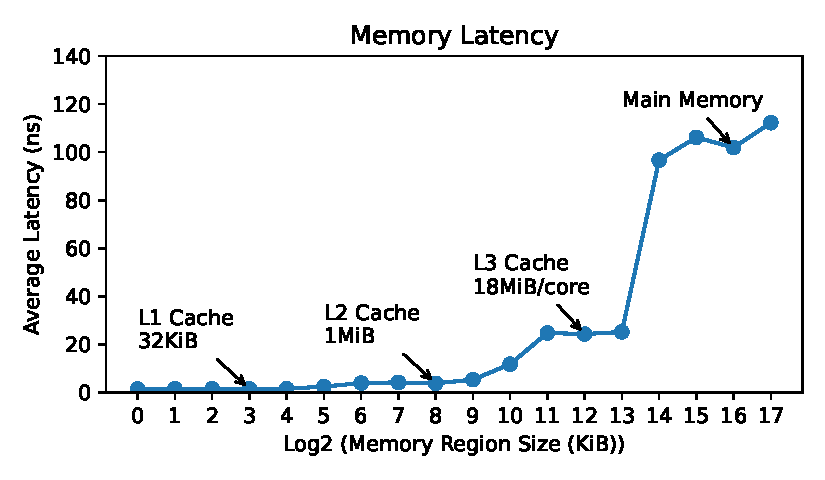
\includegraphics[width=0.98\linewidth]{sourcecode/memory/access_latency.pdf}
	\caption{\label{fig:access_lat} \textbf{RAM Access Latency}}
	%\vspace{-4mm}
\end{figure}
Figure~\ref{fig:access_lat} plots the RAM access latency result measured in our virtual machine (VM).
We can see that when we increase memory access region, the average access latency increase drastically
(from 1ns to more than 100ns). In each phase, we add a tag for current estimated access position from
L1, L2, L3, and to main memory. Experiment shows that L1 cache access latency is around 1.5ns,
L2 cache access latency is around 5ns, L3 cache access latency is around 25ns, and main memory access
latency is around 110ns.

\paragraph{Results analysis.}
For buffer sizes from 1 KiB to 32 KiB, the latency remains relatively low and consistent, suggesting these accesses are primarily served by the L1 cache. The L1 cache, being closest to the CPU and having the shortest access time, results in the lowest latency.

After a buffer size of 32 KiB, there is a noticeable increase in latency. This change is indicative of accesses beginning to spill over from the L1 cache to the L2 cache. The L2 cache, while larger than L1, has a longer access time, which results in increased latency.

As the buffer size further increases to 1024 KB and beyond, latency continues to rise. This trend is consistent with accesses reaching the L3 cache and eventually the main memory. The latency spike observed at buffer sizes of 16,384 KB and larger is particularly indicative of the transition to main memory, where access times are significantly higher than cache accesses. The main memory, being the furthest in the memory hierarchy from the CPU, exhibits the highest access latencies.

Overall, these results align with the expected behavior of our VM's memory hierarchies~\ref{table:sys-conf}. The initial low latency for smaller buffer sizes demonstrates the efficiency of CPU caches, while the increasing latency for larger sizes highlights the slower access times as data is fetched from progressively further memory layers.

\subsection{Memory Bandwidth}
\paragraph{Methodology.}
To measure the RAM bandwidth, our experiment was structured around two primary tests: reading from and writing to memory. The methodology focused on leveraging assembly language to perform these operations with minimal overhead and maximal efficiency. The assembly code was designed to bypass any compiler optimizations that could potentially skew the results.

For the read bandwidth test, a large memory block was sequentially accessed to read data, ensuring that the operation would span across the RAM's physical space. The time taken to complete this read operation was recorded. The write bandwidth test followed a similar approach, where a large memory block was sequentially written into, and the time for completion was recorded.

Both tests were conducted multiple times to account for any fluctuations in the system's state, ensuring that the results were repeatable and reliable. The average bandwidth was calculated by dividing the total size of the data transferred by the total time taken for the operation.

\paragraph{Experimental results.}
The results from the experiments are as follows:
\begin{itemize}[leftmargin=*]
	\item Read Bandwidth: 11.360022 GB/sec
	\item Write Bandwidth: 7.637086 GB/sec
\end{itemize}
These results were obtained under controlled conditions to minimize interference from other system processes.

\paragraph{Results analysis.}
The read bandwidth of 11.360022 GB/sec signifies the efficient data retrieval capability of the system's RAM. This high rate of data transfer for reading operations indicates a well-performing memory subsystem, suitable for tasks that require rapid access to large volumes of data.

On the other hand, the write bandwidth, at 7.637086 GB/sec, while lower than the read bandwidth, still reflects a strong performance. The difference in read and write speeds can be attributed to the intrinsic design of memory technologies, where writing data typically involves more complex operations than reading.

The results align with expected behavior in our VM's memory architectures, where read operations are generally faster than write operations. The significant bandwidths recorded for both read and write operations demonstrate the capability of the system's memory to handle high-demand applications and processes.

Overall, the experiment successfully showcased the system's memory bandwidth, providing valuable insights into its performance characteristics in both reading and writing operations.

\subsection{Page Fault Service Time.}
\paragraph{Methodology.}
The methodology for measuring the page fault service time involved a three-step process tailored to ensure accurate measurement of the time taken to handle a page fault, specifically focusing on the scenario where data is fetched from the disk rather than from the system's cache.

First, a large file of 5GB was created and written with data. This size was chosen to ensure that it significantly exceeds the system's total memory of 904MB, thereby guaranteeing that not all data could be cached in memory. After writing the data to the file, \emph{fsync} was used to force the file's contents to be physically written to the disk, ensuring that subsequent file accesses would indeed involve disk reads.

Second, before measuring the page fault service time, the system's buffer and cache were cleared using Linux command-line (i.e., \emph{echo 3 > /proc/sys/vm/drop\_caches}). This step was crucial to ensure that the data would indeed have to be read from the disk, triggering page faults, rather than being served from the cached memory.

Third, the function designed to measure the page fault service time was executed. This function involved accessing the data from the previously created file, thereby triggering page faults. The time taken to service these faults was recorded, providing a measure of the average service time for each page fault.

\paragraph{Experimental results.}
The average page fault service time is 0.026765 ms from our experiments.
This result represents the average time taken by the system to handle a single page fault when fetching data from the disk.

\paragraph{Results analysis.}
The average page fault service time of 0.026765 ms indicates the efficiency of the system's disk-based paging mechanism. Considering the limited total memory of 904MB~\ref{table:sys-conf} and the use of a 5GB file, the system was compelled to frequently access the disk to retrieve data not present in memory, leading to numerous page faults.

Dividing by the size of a page, it is much higher than accessing a byte from main memory as we measured before.
The relatively low page fault service time under these conditions suggests a reasonably swift disk access speed and an efficient page handling mechanism by the operating system. It is worth noting that page fault service times can be significantly influenced by various factors, including disk speed, the efficiency of the operating system's paging algorithms, and the overall system load.

In summary, the experiment effectively demonstrates the system's capability to handle page faults, providing a quantifiable measure of the time taken to retrieve data from the disk under conditions that simulate a memory-intensive workload. This insight is particularly valuable for understanding the system's performance in scenarios where the working set size exceeds the available physical memory.
\section{Network}
In this section, we will measure round trip time, peak bandwidth, and connection overhead, respectively. All the spec of our machines are identical to the previous sections.

\subsection{Round Trip Time.}
\paragraph{Methodology.} Round trip time (RTT) is the duration it takes for a network request to go from a starting point to a destination and back again to the starting point. To measure Round trip time, we setup two identical machines. We use TCP protocol in this section.

5-layer model consists Physical layer, Data Link Layer, Network Layer, Transport Layer, and Application Layer. Since we use TCP protocol we only care about physical, data link, network and transport layer as the Application layer is built upon Transport layer where TCP lives in. Thus the RTT mainly consists delays in data links and physical transmissions and packet parsing in Network and Transport layer. We measure the RTT at the client's side by timing before sending a packet and after receiving the reply.

\paragraph{Experimental results.}
We send 256 packets sequentially. The results are as follows:
\begin{itemize}[leftmargin=*]
	\item remote interface: 0.394531 ms
	\item loopback: 0.042969 ms
\end{itemize}
We also test with \texttt{ping} command:
\begin{itemize}[leftmargin=*]
	\item remote interface: 0.345 ms
	\item loopback: 0.031 ms
\end{itemize}
Our results are very close to \texttt{ping}.

\paragraph{Results analysis.} Obviously RTT of loopback is significantly smaller than remote interface. Not only because there is no network transmission delay but also related to the loopback device. 

Loopback device is a special device that the machine uses to communicate with itself. Loopback device is a virtual device which means there is no real physical interface of it. It does not represent any physical device. Loopback device is designed to make any applications on one machine can always connect to the same machine even when the network is down.

In Linux kernel, \texttt{loopback\_net\_init()} will initilize the virtual loopback NIC \texttt{lo} by \texttt{alloc\_netdev(0, "lo", NET\_NAME\_PREDICTABLE, loopback\_setup);}. The ops structure \texttt{loopback\_ops} specifies \texttt{loopback\_xmit} to perform xmit action. \texttt{loopback\_xmit} won't perform any special processing to the socket buffer (\texttt{struct sk\_buf}). Thus it is possible to omit some of the transport layer and all of the network layer logic when sending packet to loopback address. But loopback driver still use \texttt{\_\_netif\_rx()} to send the packet thus Linux still need to go  through the transport layer and network layer. Sending packet to loopback driver also means there is no delay in Physical and Data Link layer since we won't really send out the packet. In other words, RTT of loopback can be close to the baseline of network performance, with 0 delay in physical transmission.

Notice that the RTT of \texttt{ping} is actually slightly less than our result. This could be related to the ICMP protocol. ICMP packet doesn't rely on TCP protocol. In our implementation the packet is sent with TCP protocol thus there can be overhead of TCP packet processing or possible re-transmission.

\subsection{Peak Bandwidth.} 
\paragraph{Methodology.} Network bandwidth refers to the data transfer rate or capacity of a given network. It typically represents the amount of data that can be transmiited over the network in a given time frame. Higher bandwidth allows for faster data transfer and better performances in network activities including downloading or uploading files. 

To measure the peak bandwidth we need to figure out when it can reach its peak performance. For a data link with higher latency, larger TCP window size can reach better throughput in general. Since TCP protocal requires implicit ACK for a sent packet thus larger window means less packet sending and less time spent on waiting for reply. We can inspect the window size with \texttt{/proc/sys/net/ipv4/tcp\_rmem} and \texttt{/proc/sys/net/ipv4/tcp\_wmem}. However it doesn't always work since larger window means greater possibility to raise out-of-memory problem. The optimal window size can be represented as
\begin{equation}
W=L_{\text{link}} \times t_{\text{RTT}}
\end{equation}
where $L_{\text{link}}$ denotes the capacity of the link. So the optimal window size of our instances is approximately $200000$ bytes. We implemented a C-S style testing suite. The client sends message to the server and then the server replies, the client then receives the reply and we calculate the time required to send and receive the reply on the client side.

\paragraph{Experimental results.}
We send $10 \times 256 \times 80000$ bytes and here is the results:
\begin{itemize}[leftmargin=*]
	\item remote upload:    671475409 Bytes/s
	\item remote download: 1678688524 Bytes/s
\end{itemize}
\begin{itemize}[leftmargin=*]
	\item loopback upload:   3432678465 Bytes/s
	\item loopback download: 3947580235 Bytes/s
\end{itemize}
\paragraph{Results analysis.} As we noted previously, loopback packet will be handled by the loopback driver. So upload and download bandwidth of loopback should be almost the same. 

Although the bandwidth of our instance in AWS's documentation is 5Gbps, AWS features burstable bandwidth that allows user to exceed maximum bandwidth for a while if data transmission is on high demand. Also, ENA Express can let instances within the same subnet to achieve up to 25 Gbps between those instances\cite{amazonec2}. This is aligned with our experimental results. Also since we are conducting experiments with two AWS instances, the performance here refers to the internal network bandwidth of the AWS instance.

\subsection{Connection Overhead.} 
\paragraph{Methodology.} The major part of connection overhead comes from connection setup and tearing down. 

In Linux kernel, connect system call actually invokes the ops of the kernel internal structure \texttt{struct socket}, as well as other socket operations. For TCP connection it will call into \texttt{\_\_inet\_stream\_connect} and then handles the connection follows to the TCP protocol. Similarly, \texttt{shutdown} goes into \texttt{inet\_shutdown}. Those system calls handle all userland needs for setting up or tearing down a TCP connection. Thus we only need to measure the overhead of these system calls to get the overhead of connection.

Note that although the port won't be released immediately after \texttt{close()} instead it will be set to \texttt{TIME\_WAIT} mode, this won't affect our result since the communication channel is still closed. We calculate the time it takes to \texttt{connect()}, \texttt{close()}, and \texttt{shutdown()}.

\paragraph{Experimental results.} The average connection overhead of 256 times connection is 9966999 cycles. To reduce the overhead during packet transmission, we connect to the loopback address since the packet will be handled by the loopback driver.

\paragraph{Results analysis.} The results are consists of two parts: kernel space and userland. Connect setting up happens in kernel space while user needs to switch into kernel by system call. Thus syscall overhead and context switching are also included in connection overhead. By subtracting syscall cycles from the results we can have the average connection overhead is approximately $9965545.367$ cycles.

From the previous analysis, the main components of the RTT of sending packet to loopback address are the connection overhead and the processing time of the packet in the protocol layers. After getting the connection overhead, we can derive the overhead of packet processing in network layer by
\begin{equation}
    t_{packet\ processing}=t_{RTT\ loopback}-t_{connection\ overhead}
\end{equation}
This can represent the baseline overhead of TCP packet processing go through different layers in the protocol.

\section{File System}
\label{sec:file}
In this section, we will measure file system including file cache, file read time, remote file read time, and contention.

\subsection{Size of File Cache}
\paragraph{Methodology.}
The methodology of this experiment is centered around the evaluation of how file cache size, managed by the operating system, affects file read I/O time. This was done through a custom C program designed to read files of varying sizes and measure the time taken for these reads. The program systematically reads files, starting from a size of 1 KB and incrementally doubling up to 1 GB. To capture a comprehensive view, the experiment was conducted twice: first to measure the initial read times (likely with minimal cache influence), and second to measure read times when the files are expected to be cached by the OS, thus highlighting the cache's effect. 

\paragraph{Experimental results.}
\begin{figure}[t]
	\centering
	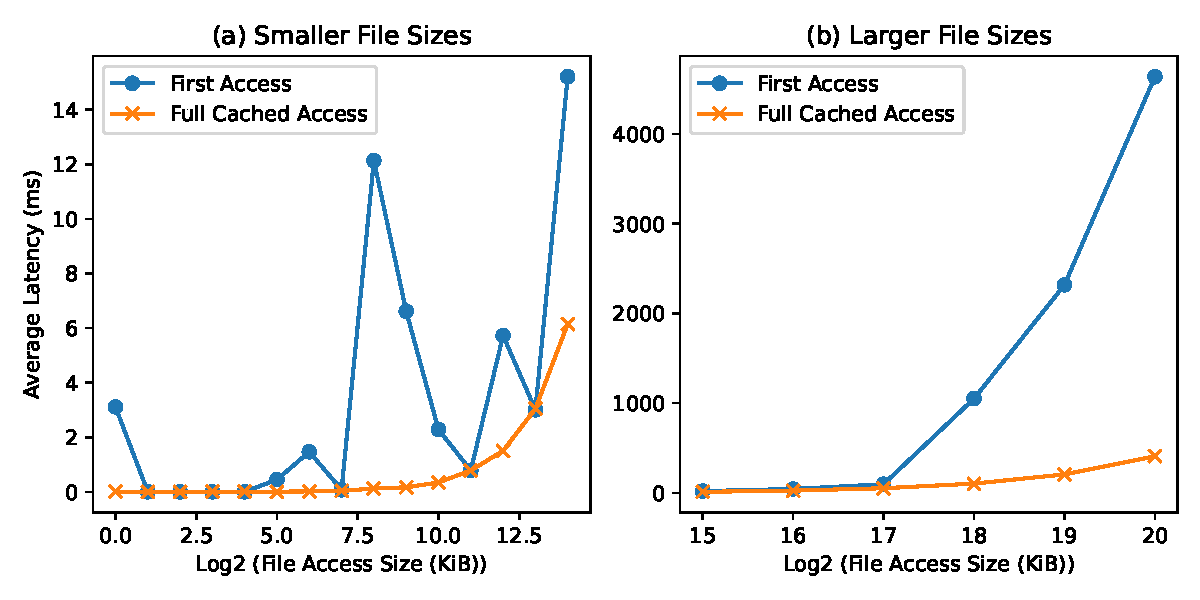
\includegraphics[width=0.98\linewidth]{sourcecode/file/filecache.pdf}
	\caption{\label{fig:file_cache} \textbf{File Cache Access}}
	%\vspace{-4mm}
\end{figure}
Figure~\ref{fig:file_cache} shows the results of file access time with increasing file access size. Since small file access and large file access show pretty different latencies. We split the results into two figures. Figure~\ref{fig:file_cache}(a) plots results under smaller file access sizes (from 1KiB to 8MiB) while Figure~\ref{fig:file_cache}(b) plots results under larger file access sizes (from 8MiB to 1GiB). By observing difference between first access (i.e., non-fully cached) and second access (i.e., full cached access), we can see the notable influence by OS file page cache. In full cached file access, the latencies are lower and more stable compared to first access (i.e., non-fully cached).

\paragraph{Results analysis.}
The analysis of the results underscores the significant role of the file system cache in optimizing read operations, especially as file sizes increase. For smaller files, the impact of caching is less pronounced, likely due to the lower overall read time. However, as file sizes grow, the benefits of caching become increasingly evident. The experiment highlights how the operating system dynamically allocates memory for caching, efficiently managing resources to balance performance with other system demands. This dynamic allocation is key in handling varying workloads, as seen in the significant improvement in read times for large, cached files. The results provide valuable insights into the behavior of file system caches and underscore their importance in system performance optimization, especially for applications dealing with large-scale file operations.

\subsection{File Read Time}
\paragraph{Methodology.}
The experimental methodology was designed to evaluate the average read times for 4 KB pages within an increasingly larger file access range, expanding from 4 KB to 1 GB. The aim was to reveal how the read times are affected as the file size grows, especially contrasting the behaviors of sequential and random access. In sequential reads, the access pattern remains linear irrespective of the file size, potentially benefiting from consistent data retrieval strategies. For random reads, the expansion in the file access range introduces more variability and randomness in access locations, expected to exhibit a more pronounced effect on read times due to increased randomness and seek times in larger files.

\paragraph{Experimental results.}
\begin{figure}[t]
	\centering
	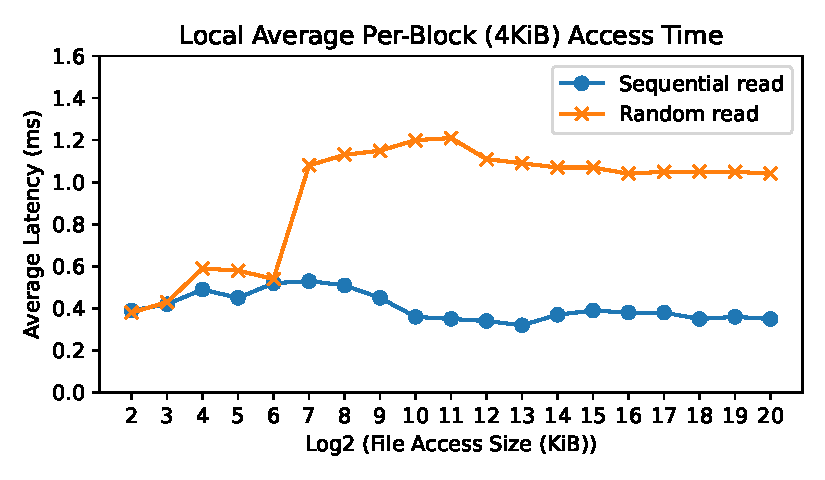
\includegraphics[width=0.98\linewidth]{sourcecode/file/file_direct.pdf}
	\caption{\label{fig:file_read_time} \textbf{File Read Time}}
	%\vspace{-4mm}
\end{figure}
Figure~\ref{fig:file_contention} plots the results of file read time with increasing file access region size.
The results show that with the increase in file size, the latency for sequential reads remain relatively stable with a slight decrease, suggesting a consistently efficient access pattern across various file sizes. In contrast, the read times for random access exhibits a notable increase as the file access range grew. This trend is more pronounced in larger file sizes, where the random nature of access leads to significantly higher read times compared to smaller sizes. The data highlight the impact of file size on read times, especially underlining the increasing inefficiency of random reads as the file size expanded.

\paragraph{Results analysis.}
These findings suggest that while sequential read operations maintain a relatively stable efficiency across different file sizes, random reads become increasingly inefficient with larger files. The stable performance of sequential reads can be attributed to the predictability and reduced seek times associated with linear data access. On the other hand, the increasing inefficiency observed in random reads for larger files is likely due to the higher seek times and the growing unpredictability in accessing data locations. This contrast in performance highlights the critical impact of file access patterns on read efficiency, particularly underlining the challenges in managing random reads in systems dealing with large files. This insight is essential for optimizing file system performance and can guide the design and optimization of data storage and retrieval strategies in large-scale data environments.

\subsection{Remote File Read Time}
\paragraph{Methodology.}
We use the same methodology and experimental program with local file read time experiment aforementioned. The only difference is that we use NFS instead of local filesystem on local disk. Therefore, we use another same virtual machine as NFS target and use our experimental to connect to NFS target. After that, we can see a NFS filesystem in our test machine. Finally, we run the same program to evaluate remote file read time on both random and sequential workloads.

\paragraph{Experimental results.}
\begin{figure}[t]
	\centering
	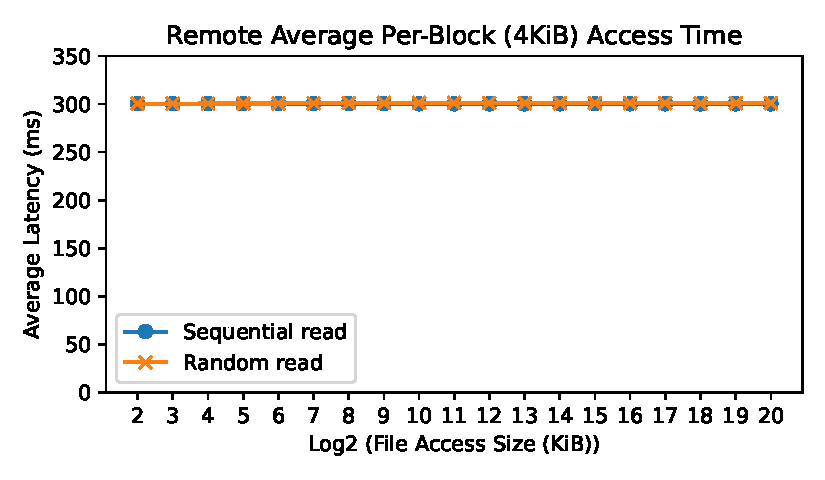
\includegraphics[width=0.98\linewidth]{sourcecode/file/file_remote.pdf}
	\caption{\label{fig:remote_file_read_time} \textbf{File Read Time}}
	%\vspace{-4mm}
\end{figure}
Figure~\ref{fig:remote_file_read_time} plots the results of remote file read time with increasing file access region size. The result is quite different with local file read time. In this remote access case, both random and sequential reads show almost same latency, which is pretty higher than local file read time. Even though we increase file access region size, the results do not show any difference.

\paragraph{Results analysis.}
From the results, we can get that reading remote file results in much higher latency than reading local file. This is because the network access time. The network access time is pretty higher than disk access time in our machines. Therefore, this leads to same access time for both sequential and random reads. This experiment tells us that in order to accelerate remote file access, both network and disk efficiency are equally important. We should optimize network and disk access efficiency together. 

\subsection{Contention}
\paragraph{Methodology.}
The experiment is designed to evaluate the concurrent read performance of a filesystem, particularly when multiple processes are simultaneously reading from different files on the same disk. The primary objective is to understand how increasing the number of processes affects the average read time for a single filesystem block. Our test program uses Direct I/O to bypass the file buffer cache, ensuring a more accurate measurement of disk access times. Each process reads 1024 blocks, each of 4096 bytes (typical filesystem block size), from a unique file. The read operations are performed randomly across the file to prevent sequential read optimizations and better mimic real-world access patterns. The experiment iterates over a varying number of processes, starting from 1 and going up to 16.
The total time taken for all reads in each process is then divided by the number of blocks to obtain the average block read time in milliseconds.

\paragraph{Experimental results.}
\begin{figure}[t]
	\centering
	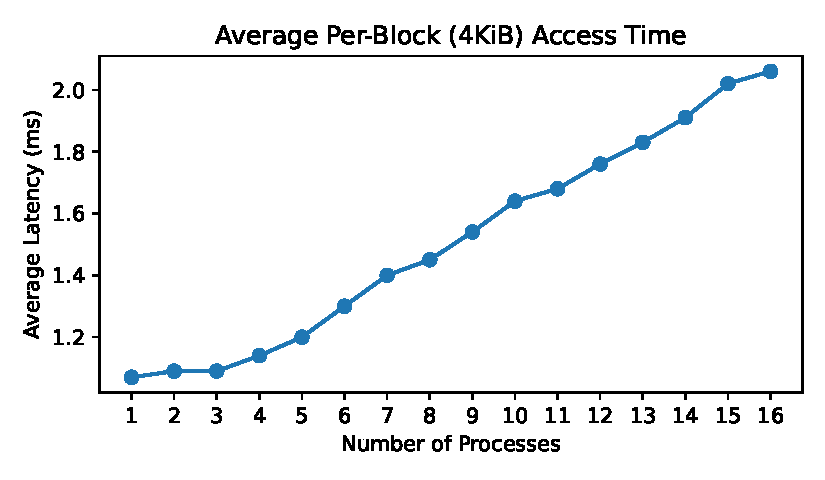
\includegraphics[width=0.98\linewidth]{sourcecode/file/file_contention.pdf}
	\caption{\label{fig:file_contention} \textbf{File Contention}}
	%\vspace{-4mm}
\end{figure}
Figure~\ref{fig:file_contention} plots the per-block (4KiB) access time under different concurrency. We can see that with the increasing of number of concurrent processes, the average per-block latency increases up to 2$\times$ (with 16 processes access simultaneously) compared to single process access.

\paragraph{Results analysis.}
The data indicates a clear trend: as the number of concurrent processes increases, the average time taken to read a single block also increases. This result is consistent with expectations, as more processes lead to increased contention for disk resources.

In the initial stages (1-4 processes), the increase in read time is relatively marginal, suggesting that the disk subsystem can handle low levels of concurrency without significant degradation in performance. However, beyond 4 processes, the read time starts increasing at a higher rate. This trend is more pronounced from 9 processes onwards, indicating a substantial contention in the disk subsystem.
\clearpage
\bibliographystyle{plainurl}
\bibliography{bibliography}

%\clearpage
%\appendix
%\input{appendix}
\end{document}

